\chapter{Di Dalam Atom}\label{ch:g9:inside-the-atom}

Pada tahun 1909, di sebuah laboratorium di Manchester, seberkas partikel
yang sangat kecil dan cepat ditembakkan ke selembar emas tipis yang
tebalnya hanya beberapa ratus \omterm{def:g7:atoms-and-molecules:atom}{atom}. Hampir semuanya lewat lurus, seolah
emas itu kosong. Tetapi sekitar satu dari beberapa ribu partikel
memantul kembali. ``Seolah-olah kamu menembakkan peluru meriam 15 inci
ke selembar kertas tisu, lalu peluru itu berbalik dan mengenaimu,''
kata Ernest Rutherford, yang murid-muridnya melakukan percobaan itu.
\omterm{def:g7:atoms-and-molecules:atom}{Atom}, kepingan materi yang tak terpotong, ternyata memiliki struktur ---
dan hampir seluruhnya kosong.

\begin{recall}
Semua materi tersusun atas \omterm{def:g7:atoms-and-molecules:atom}{atom}, dengan sekitar seratus jenis yang
berbeda, masing-masing dengan lambang seperti \ce{H}, \ce{C}, \ce{O},
\ce{Fe}. \omterm{def:g7:atoms-and-molecules:atom}{Atom-atom} bergabung menjadi \omterm{def:g7:atoms-and-molecules:molecule}{molekul}, yang dinyatakan dengan
rumus seperti \ce{H2O} (\cref{ch:g7:atoms-and-molecules}).
\end{recall}

\section{Inti atom dan elektron}

\begin{definition}[Inti atom dan elektron]\label{def:g9:inside-the-atom:nucleus}
Setiap \omterm{def:g7:atoms-and-molecules:atom}{atom} memiliki pusat yang sangat kecil dan berat, yaitu
\emph{inti atom}\index{inti atom}, yang bermuatan listrik positif. Di
sekelilingnya bergerak partikel-partikel yang jauh lebih ringan, yaitu
\emph{elektron}\index{elektron}, yang masing-masing membawa muatan
negatif yang sama, $-e$.
\end{definition}

\begin{proposition}[Atom itu netral]\label{prop:g9:inside-the-atom:neutral}
% ledger: const:e
Sebuah \omterm{def:g7:atoms-and-molecules:atom}{atom} secara keseluruhan tidak bermuatan listrik: muatan positif
intinya tepat diimbangi oleh muatan negatif \omterm{def:g9:inside-the-atom:nucleus}{elektron-elektronnya}.
Muatan $e$ sangat kecil: $e = \qty{1.60e-19}{C}$ (coulomb, satuan
muatan, dibahas di buku fisika).
\end{proposition}

\begin{omfigure}
\begin{tikzpicture}[font=\small]
  \shade[inner color=omDef!35, outer color=white] (0,0) circle (2.2);
  \draw[omDef!60, dashed] (0,0) circle (2.2);
  \foreach \a/\r in {20/1.6,95/1.1,150/1.9,215/1.4,290/1.7,340/0.9} {
    \fill[omDef] (\a:\r) circle (0.06);
    \node[font=\scriptsize, omDef] at ($(\a:\r)+(0.18,0.16)$) {$-$};
  }
  \fill[red!70!black] (0,0) circle (0.1);
  \draw[<-, omProp, thick] (-0.12,0.02) -- (-3.0,0.9) node[left, text=black, align=right]
    {inti atom: sangat kecil,\\ berat, positif};
  \draw[<-, omProp, thick] ($(20:1.6)+(0.08,0.02)$) -- (3.0,0.9) node[right, text=black]
    {sebuah elektron: ringan, negatif};
  \draw[<-, omProp, thick] (300:2.2) -- (3.0,-1.4) node[right, text=black, align=left]
    {elektron-elektron bergerak dalam awan\\ di sekeliling inti};
\end{tikzpicture}

{\small Sebuah \omterm{def:g7:atoms-and-molecules:atom}{atom}, tidak menurut skala. Jika inti digambar sebesar
titik merah itu, awan \omterm{def:g9:inside-the-atom:nucleus}{elektronnya} akan berukuran beberapa ratus meter.}
\end{omfigure}

\section{Proton dan neutron}

\begin{definition}[Proton, neutron, nukleon]\label{def:g9:inside-the-atom:proton}
\omterm{def:g9:inside-the-atom:nucleus}{Inti atom} tersusun atas dua jenis partikel: \emph{proton}\index{proton},
yang masing-masing bermuatan $+e$, dan \emph{neutron}\index{neutron},
yang tidak bermuatan. Proton dan neutron, yang massanya hampir sama,
bersama-sama disebut \emph{nukleon}\index{nukleon}.
\end{definition}

\begin{definition}[Nomor atom dan nomor massa]\label{def:g9:inside-the-atom:atomic-number}
Banyaknya \omterm{def:g9:inside-the-atom:proton}{proton} dalam sebuah inti disebut
\emph{nomor atom}\index{nomor atom}, ditulis $Z$. Banyaknya \omterm{def:g9:inside-the-atom:proton}{nukleon}
(\omterm{def:g9:inside-the-atom:proton}{proton} dan \omterm{def:g9:inside-the-atom:proton}{neutron} bersama-sama) disebut
\emph{nomor massa}\index{nomor massa}, ditulis $A$. Banyaknya \omterm{def:g9:inside-the-atom:proton}{neutron}
adalah $N = A - Z$.
\end{definition}

\begin{notation}[Lambang nuklida]\label{not:g9:inside-the-atom:symbol}
\omterm{def:g7:atoms-and-molecules:atom}{Atom} dengan inti tertentu ditulis dengan lambangnya, \omterm{def:g9:inside-the-atom:atomic-number}{nomor massa} di
kiri atas dan \omterm{def:g9:inside-the-atom:atomic-number}{nomor atom} di kiri bawah: \ce{^{A}_{Z}X}. Misalnya
\ce{^{12}_{6}C} memiliki 6 \omterm{def:g9:inside-the-atom:proton}{proton} dan $12 - 6 =
6$ \omterm{def:g9:inside-the-atom:proton}{neutron}; \ce{^{56}_{26}Fe} memiliki 26 \omterm{def:g9:inside-the-atom:proton}{proton} dan 30 \omterm{def:g9:inside-the-atom:proton}{neutron}.
\end{notation}

\begin{method}[Membaca lambang nuklida]\label{met:g9:inside-the-atom:read}
Untuk \ce{^{A}_{Z}X}:
\begin{enumerate}
  \item \omterm{def:g9:inside-the-atom:proton}{proton}: $Z$;
  \item \omterm{def:g9:inside-the-atom:proton}{neutron}: $A - Z$;
  \item \omterm{def:g9:inside-the-atom:nucleus}{elektron} \omterm{def:g7:atoms-and-molecules:atom}{atom} netral: $Z$, sama dengan \omterm{def:g9:inside-the-atom:proton}{protonnya}.
\end{enumerate}
Untuk \ce{^{23}_{11}Na}: 11 \omterm{def:g9:inside-the-atom:proton}{proton}, 12 \omterm{def:g9:inside-the-atom:proton}{neutron}, 11 \omterm{def:g9:inside-the-atom:nucleus}{elektron}.
\end{method}

\begin{omfigure}
\begin{tikzpicture}[font=\small]
  \node[font=\Huge, inner sep=1pt] (x) at (0,0) {\ce{^{35}_{17}Cl}};
  \draw[<-, omProp, thick, shorten <=3pt] ([xshift=5pt,yshift=-7pt]x.north west) -- (-2.6,1.0)
    node[left, text=black, align=right] {nomor massa $A = 35$:\\ proton + neutron};
  \draw[<-, omProp, thick, shorten <=3pt] ([xshift=5pt,yshift=7pt]x.south west) -- (-2.6,-1.0)
    node[left, text=black, align=right] {nomor atom $Z = 17$:\\ proton};
  \draw[<-, omProp, thick] ([xshift=2pt]x.east) -- (2.2,0) node[right, text=black,
    align=left] {lambang unsur:\\ klorin};
\end{tikzpicture}

{\small Membaca lambang nuklida: \omterm{def:g7:atoms-and-molecules:atom}{atom} klorin ini memiliki 17 \omterm{def:g9:inside-the-atom:proton}{proton},
$35 - 17 = 18$ \omterm{def:g9:inside-the-atom:proton}{neutron}, dan 17 \omterm{def:g9:inside-the-atom:nucleus}{elektron} dalam keadaan netral.}
\end{omfigure}

\section{Unsur kimia dan isotopnya}

\begin{definition}[Unsur kimia]\label{def:g9:inside-the-atom:element}
Yang disebut \emph{unsur kimia}\index{unsur kimia} adalah himpunan semua
\omterm{def:g7:atoms-and-molecules:atom}{atom}, beserta semua \omterm{def:g7:atoms-and-molecules:atom}{atom} bermuatan yang terbentuk darinya, yang memiliki
\omterm{def:g9:inside-the-atom:atomic-number}{nomor atom} $Z$ yang sama. Setiap unsur memiliki nama dan lambang: setiap
\omterm{def:g7:atoms-and-molecules:atom}{atom} dengan 6 \omterm{def:g9:inside-the-atom:proton}{proton} adalah \omterm{def:g7:atoms-and-molecules:atom}{atom} karbon, \ce{C}; setiap \omterm{def:g7:atoms-and-molecules:atom}{atom} dengan 8
\omterm{def:g9:inside-the-atom:proton}{proton} adalah \omterm{def:g7:atoms-and-molecules:atom}{atom} oksigen, \ce{O}.
\end{definition}

\begin{definition}[Isotop]\label{def:g9:inside-the-atom:isotope}
\omterm{def:g7:atoms-and-molecules:atom}{Atom-atom} dari unsur yang sama yang banyak \omterm{def:g9:inside-the-atom:proton}{neutronnya} berbeda, sehingga
\omterm{def:g9:inside-the-atom:atomic-number}{nomor massanya} berbeda, disebut \emph{isotop}\index{isotop} unsur itu.
Isotop-isotop itu memiliki $Z$ yang sama dan $A$ yang berbeda.
\end{definition}

\begin{example}[Isotop karbon dan isotop hidrogen]\label{ex:g9:inside-the-atom:isotopes}
% ledger: iso:C12, iso:C13, iso:H2
Karbon alami terdiri atas sekitar \qty{98.9}{\percent} karbon-12,
\ce{^{12}_{6}C}, dan \qty{1.1}{\percent} karbon-13, \ce{^{13}_{6}C},
dengan sedikit sekali karbon-14, \ce{^{14}_{6}C}, yang perubahannya
yang lambat menjadi inti lain dipakai untuk menentukan umur kayu dan
tulang purba (keradioaktifan dibahas di buku fisika). Hidrogen memiliki
tiga \omterm{def:g9:inside-the-atom:isotope}{isotop}: \ce{^{1}_{1}H}, tanpa \omterm{def:g9:inside-the-atom:proton}{neutron} sama sekali, yang paling
umum; deuterium \ce{^{2}_{1}H}, beberapa \omterm{def:g7:atoms-and-molecules:atom}{atom} dalam setiap seratus ribu;
dan tritium \ce{^{3}_{1}H}.
\end{example}

\begin{proposition}[Isotop-isotop berperilaku sama dalam kimia]\label{prop:g9:inside-the-atom:alike}
Sifat kimia sebuah \omterm{def:g7:atoms-and-molecules:atom}{atom} bergantung pada \omterm{def:g9:inside-the-atom:nucleus}{elektron-elektronnya}, dan
\omterm{def:g9:inside-the-atom:isotope}{isotop-isotop} sebuah unsur memiliki jumlah \omterm{def:g9:inside-the-atom:nucleus}{elektron} yang sama. Karena
itu \omterm{def:g9:inside-the-atom:isotope}{isotop-isotop} bereaksi dengan cara yang sama: air yang dibuat
dengan deuterium tampak dan berperilaku hampir persis seperti air
biasa.
\end{proposition}

\begin{omfigure}
\begin{tikzpicture}[font=\small, p/.style={circle, inner sep=0pt, minimum size=4.2mm,
    ball color=red!65}, n/.style={circle, inner sep=0pt, minimum size=4.2mm,
    ball color=black!20}]
  \node[p] at (0,0) {};
  \node[anchor=north, align=center] at (0,-0.45) {\ce{^{1}_{1}H}\\ 1 proton};
  \node[p] at (3.0,0) {}; \node[n] at (3.35,0.1) {};
  \node[anchor=north, align=center] at (3.2,-0.45) {\ce{^{2}_{1}H}\\ 1 proton, 1 neutron};
  \node[p] at (6.4,0) {}; \node[n] at (6.75,0.12) {}; \node[n] at (6.55,0.35) {};
  \node[anchor=north, align=center] at (6.6,-0.45) {\ce{^{3}_{1}H}\\ 1 proton, 2 neutron};
  \node[draw=black!30, fill=red!65, circle, minimum size=3mm, inner sep=0pt] at (9.1,0.2) {};
  \node[anchor=west] at (9.3,0.2) {proton};
  \node[draw=black!30, fill=black!20, circle, minimum size=3mm, inner sep=0pt] at (9.1,-0.3) {};
  \node[anchor=west] at (9.3,-0.3) {neutron};
\end{tikzpicture}

{\small Inti ketiga \omterm{def:g9:inside-the-atom:isotope}{isotop} hidrogen: masing-masing satu \omterm{def:g9:inside-the-atom:proton}{proton}, dan 0, 1,
atau 2 \omterm{def:g9:inside-the-atom:proton}{neutron}.}
\end{omfigure}

\section{Ukuran dan massa}

\begin{proposition}[Inti atom sangat kecil dan memuat hampir seluruh massa]\label{prop:g9:inside-the-atom:sizes}
% ledger: const:a0, r:proton, const:mp, const:mn, const:me
Sebuah \omterm{def:g7:atoms-and-molecules:atom}{atom} berukuran sekitar \qty{e-10}{m}; intinya, sekitar
\qty{e-15}{m} sampai \qty{e-14}{m}: kira-kira sepuluh ribu sampai seratus
ribu kali lebih kecil. Massa partikel-partikelnya adalah
\[
  m_p = \qty{1.673e-27}{kg},\qquad m_n = \qty{1.675e-27}{kg},\qquad
  m_e = \qty{9.11e-31}{kg}.
\]
Sebuah \omterm{def:g9:inside-the-atom:proton}{proton} kira-kira 1836 kali lebih berat daripada sebuah \omterm{def:g9:inside-the-atom:nucleus}{elektron},
sehingga lebih dari \qty{99.9}{\percent} massa sebuah \omterm{def:g7:atoms-and-molecules:atom}{atom} berada di
intinya.
\end{proposition}

\begin{example}[Kelereng di tengah stadion]\label{ex:g9:inside-the-atom:marble}
Jika inti sebuah \omterm{def:g7:atoms-and-molecules:atom}{atom} adalah kelereng berdiameter \qty{1}{cm}, \omterm{def:g7:atoms-and-molecules:atom}{atomnya}
akan berdiameter sekitar $\qty{1}{cm} \times 100\,000 = \qty{1}{km}$:
sebutir kelereng di tengah stadion raksasa, dengan beberapa butir debu
--- \omterm{def:g9:inside-the-atom:nucleus}{elektron-elektronnya} --- berputar-putar di sekitar tribun. Materi
sebagian besar berupa ruang kosong.
\end{example}

\begin{method}[Massa sebuah atom]\label{met:g9:inside-the-atom:mass}
Karena \omterm{def:g9:inside-the-atom:proton}{proton} dan \omterm{def:g9:inside-the-atom:proton}{neutron} hampir sama massanya dan \omterm{def:g9:inside-the-atom:nucleus}{elektron} sangat
ringan, massa sebuah \omterm{def:g7:atoms-and-molecules:atom}{atom} mendekati $A \times
\qty{1.67e-27}{kg}$, dengan $A$ \omterm{def:g9:inside-the-atom:atomic-number}{nomor massanya}. Sebuah \omterm{def:g7:atoms-and-molecules:atom}{atom} karbon-12:
$12 \times 1.67 \times 10^{-27} = \qty{2.00e-26}{kg}$.
\end{method}

\section{Sejarah singkat model atom}

\begin{history}[Dari yang tak terpotong sampai inti atom, 1897--1932]
Pada tahun 1897 J.~J.~Thomson menemukan \omterm{def:g9:inside-the-atom:nucleus}{elektron}, partikel yang jauh
lebih ringan daripada \omterm{def:g7:atoms-and-molecules:atom}{atom} mana pun: ternyata \omterm{def:g7:atoms-and-molecules:atom}{atom} dapat dipotong. Ia
membayangkan \omterm{def:g7:atoms-and-molecules:atom}{atom} sebagai bola materi positif yang bertaburan
\omterm{def:g9:inside-the-atom:nucleus}{elektron}. Pada 1909--1911 percobaan lembaran emas oleh tim Rutherford
menunjukkan bahwa muatan positif dan hampir seluruh massa berada di
dalam inti yang sangat kecil. Pada tahun 1913 Niels Bohr mengusulkan
bahwa \omterm{def:g9:inside-the-atom:nucleus}{elektron-elektron} menempati tingkat-tingkat energi tertentu di
sekeliling inti, dan pada tahun 1932 James Chadwick menemukan \omterm{def:g9:inside-the-atom:proton}{neutron}.
\end{history}

\begin{omfigure}
\begin{minipage}[b]{0.3\linewidth}\centering
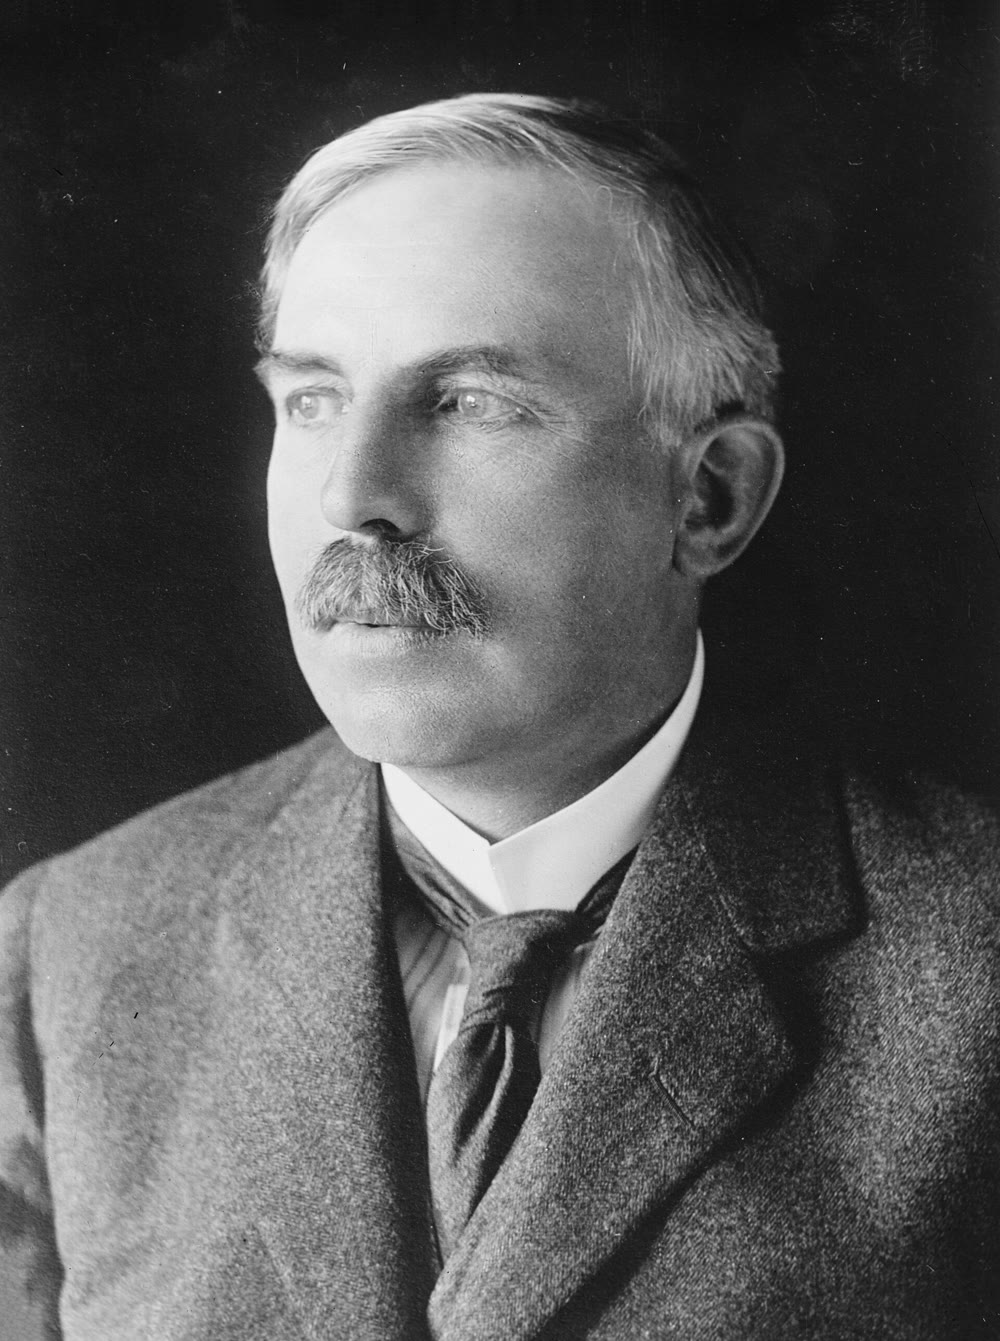
\includegraphics[width=\linewidth]{images/book1/rutherford.jpg}

{\small Ernest Rutherford (1871--1937).}
\end{minipage}\hfill
\begin{minipage}[b]{0.66\linewidth}\centering
\begin{tikzpicture}[font=\small]
  \fill[black!45] (0,-0.5) rectangle (0.9,0.5);
  \node[anchor=north, align=center] at (0.45,-0.55) {sumber\\ partikel alfa};
  \draw[->, thick, red!70!black] (0.9,0) -- (2.8,0);
  \fill[yellow!70!orange] (2.8,-1.6) rectangle (2.88,1.6);
  \node[anchor=north] at (2.84,-1.65) {lembaran emas};
  \draw[omDef!40, line width=4pt] (5.6,-1.8) arc[start angle=-30, end angle=30, radius=3.6];
  \foreach \y in {-0.3,-0.1,0.1,0.3} \draw[->, red!70!black] (2.88,\y) -- (5.3,\y);
  \draw[->, red!70!black] (2.88,0.05) -- (5.0,1.15);
  \draw[->, red!70!black] (2.88,-0.05) -- (4.9,-1.3);
  \draw[->, red!70!black, thick] (2.8,0.02) .. controls (2.2,0.35) .. (1.6,0.95);
  \node[anchor=west, align=left, font=\footnotesize] at (6.25,0) {sebagian\\ besar\\ lewat lurus};
  \node[anchor=south, align=center, font=\footnotesize] at (1.6,1.0) {sedikit sekali\\ yang memantul};
\end{tikzpicture}

{\small Percobaan lembaran emas: sebagian besar partikel lewat lurus;
beberapa dibelokkan; sedikit sekali yang memantul kembali dari sebuah
inti.}
\end{minipage}
\end{omfigure}

\section{Latihan}

\begin{exercise}[$\star$]\label{exo:g9:inside-the-atom:1}
Sebutkan partikel-partikel di dalam inti dan partikel-partikel di
sekelilingnya, beserta tanda muatannya.
\end{exercise}

\begin{exercise}[$\star$]\label{exo:g9:inside-the-atom:2}
Tentukan banyaknya \omterm{def:g9:inside-the-atom:proton}{proton}, \omterm{def:g9:inside-the-atom:proton}{neutron}, dan \omterm{def:g9:inside-the-atom:nucleus}{elektron} pada \ce{^{16}_{8}O},
\ce{^{27}_{13}Al}, dan \ce{^{40}_{20}Ca}.
\end{exercise}

\begin{exercise}[$\star$]\label{exo:g9:inside-the-atom:3}
Mengapa sebuah \omterm{def:g7:atoms-and-molecules:atom}{atom} netral secara listrik?
\end{exercise}

\begin{exercise}[$\star$]\label{exo:g9:inside-the-atom:4}
Sebuah \omterm{def:g7:atoms-and-molecules:atom}{atom} memiliki 26 \omterm{def:g9:inside-the-atom:proton}{proton} dan 30 \omterm{def:g9:inside-the-atom:proton}{neutron}. Tuliskan lambang
nuklidanya (unsurnya besi, \ce{Fe}).
\end{exercise}

\begin{exercise}[$\star\star$]\label{exo:g9:inside-the-atom:5}
Apakah \ce{^{35}_{17}Cl} dan \ce{^{37}_{17}Cl} unsur yang sama? Apakah
keduanya \omterm{def:g9:inside-the-atom:isotope}{isotop}? Jelaskan.
\end{exercise}

\begin{exercise}[$\star\star$]\label{exo:g9:inside-the-atom:6}
Apakah \ce{^{14}_{6}C} dan \ce{^{14}_{7}N} \omterm{def:g9:inside-the-atom:isotope}{isotop}? Jelaskan.
\end{exercise}

\begin{exercise}[$\star\star$]\label{exo:g9:inside-the-atom:7}
Hitung, dalam notasi ilmiah, perkiraan massa sebuah \omterm{def:g7:atoms-and-molecules:atom}{atom}
\ce{^{56}_{26}Fe}.
\end{exercise}

\begin{exercise}[$\star\star$]\label{exo:g9:inside-the-atom:8}
Dalam percobaan lembaran emas, mengapa sebagian besar partikel lewat
lurus menembus emas?
\end{exercise}

\begin{exercise}[$\star\star$]\label{exo:g9:inside-the-atom:9}
Berapa kali lebih kecil sebuah inti \qty{e-15}{m} dibandingkan sebuah
\omterm{def:g7:atoms-and-molecules:atom}{atom} (\qty{e-10}{m})? Tuliskan jawabannya sebagai perpangkatan
sepuluh.
\end{exercise}

\begin{exercise}[$\star\star$]\label{exo:g9:inside-the-atom:10}
Mengapa \omterm{def:g9:inside-the-atom:isotope}{isotop-isotop} sebuah unsur memiliki sifat kimia yang sama?
\end{exercise}

\begin{exercise}[$\star\star\star$]\label{exo:g9:inside-the-atom:11}
Sebuah \omterm{def:g7:atoms-and-molecules:atom}{atom} besi memiliki 26 \omterm{def:g9:inside-the-atom:nucleus}{elektron}. Hitung massa totalnya, lalu
bagian massa \omterm{def:g7:atoms-and-molecules:atom}{atom} \ce{^{56}_{26}Fe} yang merupakan massa \omterm{def:g9:inside-the-atom:nucleus}{elektron-elektron}
itu (pakailah massa yang diperoleh pada latihan~7).
\end{exercise}

\begin{exercise}[$\star\star\star$]\label{exo:g9:inside-the-atom:12}
% ledger: iso:Cu63, iso:Cu65
Tembaga alami terdiri atas \qty{69.15}{\percent} tembaga-63 dan
\qty{30.85}{\percent} tembaga-65. Di antara 10\,000 \omterm{def:g7:atoms-and-molecules:atom}{atom} tembaga, berapa
\omterm{def:g7:atoms-and-molecules:atom}{atom} dari setiap \omterm{def:g9:inside-the-atom:isotope}{isotop}? Berapa rata-rata banyaknya \omterm{def:g9:inside-the-atom:proton}{nukleon} per \omterm{def:g7:atoms-and-molecules:atom}{atom}
tembaga?
\end{exercise}

\clearpage % keeps the heading with its problem box (it was stranded at a page foot)
\section{Soal: Menimbang Klorin}

\begin{problem}[{Soal akhir pekan --- dua isotop klorin, massa setiap
atomnya, dan massa rata-rata sebuah atom klorin}]
\label{pb:g9:inside-the-atom:1}
% ledger: iso:Cl35, iso:Cl37, const:me, const:mp, const:mn
Klorin alami adalah \omterm{def:g6:pure-substances-and-mixtures:mixture}{campuran} dua \omterm{def:g9:inside-the-atom:isotope}{isotop}, klorin-35 dan klorin-37: dari
1000 \omterm{def:g7:atoms-and-molecules:atom}{atom} klorin, sekitar 758 adalah klorin-35 dan 242 klorin-37.
Anggaplah massa sebuah \omterm{def:g9:inside-the-atom:proton}{nukleon} \qty{1.67e-27}{kg} dan massa sebuah
\omterm{def:g9:inside-the-atom:nucleus}{elektron} \qty{9.11e-31}{kg}. \omterm{def:g9:inside-the-atom:atomic-number}{Nomor atom} klorin adalah 17.

\medskip
\noindent\textbf{Bagian I --- Dua inti.}
\begin{enumerate}
  \item Tuliskan lambang nuklida kedua \omterm{def:g9:inside-the-atom:isotope}{isotop} itu.
  \item Tentukan banyaknya \omterm{def:g9:inside-the-atom:proton}{proton}, \omterm{def:g9:inside-the-atom:proton}{neutron}, dan \omterm{def:g9:inside-the-atom:nucleus}{elektron} masing-masing.
  \item Mengapa keduanya disebut klorin? Mengapa keduanya \omterm{def:g9:inside-the-atom:isotope}{isotop}?
  \item Akankah sampel klorin-37 bereaksi dengan natrium dengan cara yang
        sama seperti sampel klorin-35? Jelaskan.
\end{enumerate}

\medskip
\noindent\textbf{Bagian II --- Massa setiap \omterm{def:g7:atoms-and-molecules:atom}{atom}.}
\begin{enumerate}[resume]
  \item Hitung massa inti sebuah \omterm{def:g7:atoms-and-molecules:atom}{atom} klorin-35.
  \item Hitung massa ke-17 \omterm{def:g9:inside-the-atom:nucleus}{elektronnya}, dan periksa bahwa massa itu dapat
        diabaikan dibandingkan intinya.
  \item Hitung massa sebuah \omterm{def:g7:atoms-and-molecules:atom}{atom} klorin-37.
  \item Berapa \omterm{def:g7:atoms-and-molecules:atom}{atom} klorin-35 yang beratnya \qty{1}{g}? Berikan jawabannya
        dalam notasi ilmiah.
\end{enumerate}

\medskip
\noindent\textbf{Bagian III --- \omterm{def:g7:atoms-and-molecules:atom}{Atom} rata-rata.}
\begin{enumerate}[resume]
  \item Berapa persen \omterm{def:g7:atoms-and-molecules:atom}{atom} klorin yang berupa klorin-35? Klorin-37?
  \item Dalam 1000 \omterm{def:g7:atoms-and-molecules:atom}{atom} klorin alami, hitung massa total \omterm{def:g7:atoms-and-molecules:atom}{atom-atom}
        klorin-35 dan \omterm{def:g7:atoms-and-molecules:atom}{atom-atom} klorin-37.
  \item Hitung massa 1000 \omterm{def:g7:atoms-and-molecules:atom}{atom} ini.
  \item Simpulkan massa rata-rata sebuah \omterm{def:g7:atoms-and-molecules:atom}{atom} klorin.
\end{enumerate}
\end{problem}
